\chapter{提案手法の設計}
\label{chap:design}

\section{概要}
提案手法の設計を\figref{fig:system-architecture}に示す.
提案手法はコンポーネントとして\textbf{Detector},\textbf{Process Monitor},\textbf{Evacuation Module},\textbf{Data Shelter}を含む.

ランサムウェアの疑いがあるプロセスをDetectorが検出してProcess Monitorに通知する.
Process Monitorは指定されたプロセスが侵害しようとするファイルのデータを取得してEvacuation Moduleに送信する.
Evacuation ModuleはProcess Monitorから受け取ったデータを処理し,Data Shelter内に侵害対象のファイルを退避させる.

% なお,ここでいう「ファイルの侵害」とは,暗号化を行ったりランダムなデータで上書きしたりすることでファイルを利用不可能にする振る舞いを指す.
\begin{figure}[t]
  \centering
  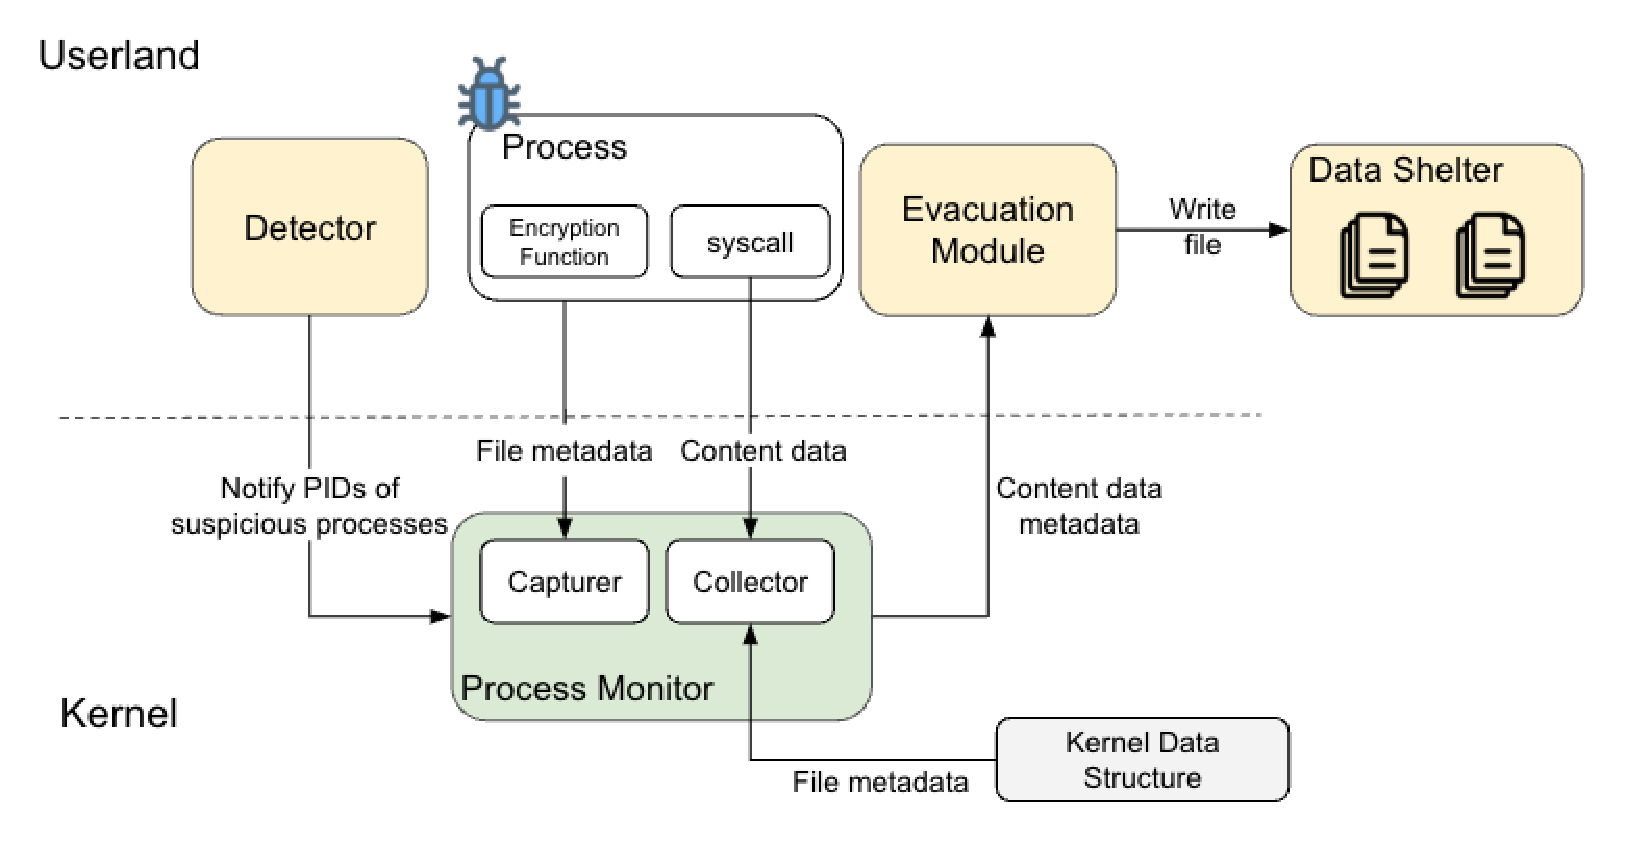
\includegraphics[width=\columnwidth]{doc/img/system_overview.eps}
  \caption{The overview of the proposed system.}
  \label{fig:system-architecture}
\end{figure}

\section{各コンポーネントの設計}
% \figref{fig:system-architecture}内の各コンポーネントをそれぞれ説明する.
\subsection{Detector}
Detectorはユーザ空間で実行されるプロセスで,自身以外のユーザプロセスを監視して保守的なランサムウェア検知を行う.
ランサムウェアの可能性が閾値よりも高いプロセスを発見した際に,そのプロセスの識別子をProcess Monitorに通知する.
一度監視対象となったがその後正常なプロセスであると判定された場合も,同様に通知を行う.
% 不審なプロセスが終了した場合も同様に通知を行う.
なお,\ref{sec:ransom-detect}節で述べたように,ランサムウェアの検知手法は先行研究が多数存在する.
したがって本研究においてDetectorの機能は利用可能であるという前提を置き,その内部実装は本研究のスコープ外とする.

\subsection{Process Monitor}
Process Monitorはカーネル空間で実行されるプログラムであり,Detectorが指定したユーザプロセスを監視している.
Process Monitorは,暗号化前の平文データを取得する\textbf{Capturer}モジュールと,
ファイルのメタデータを収集する\textbf{Collector}モジュールで構成される.
Capturerが取得した平文データとCollectorが収集したメタデータは,
一つのデータ構造に格納されてEvacuation Moduleに送信される.

Capturerは監視対象のプロセスが実行する暗号化関数をフックし,関数の引数に渡される平文データのポインタをキャプチャする.
その後ポインタが指すバッファのデータを対象のユーザプロセスのメモリ空間からカーネルメモリ空間へとコピーすることで平文データを取得する.

CollectorはCapturerと連携し,ファイルの復旧に必要なメタデータ,具体的にはファイルパスと
コンテンツデータのオフセットを以下のように収集する.
\\
ファイルパスの取得:ファイルを開くシステムコールをフックし,ファイルの相対パスをシステムコールの引数から取得する.
さらに,カーネル内構造体にアクセスして対象プロセスの現在の作業ディレクトリ(Current Working Directory: CWD)を取得する.
システムコールにはファイルの絶対パスが引数として渡されることがあるが,この場合はCWDの取得は不要となる.
% 相対パスとCWDから,操作対象のファイルの絶対パスを構成する.
\\
オフセットの取得:
あるファイルが監視対象プロセスによって開かれたら,
そのファイルのオフセットを管理する変数を初期化する.
ファイルのコンテンツデータをメモリ上に読み込むシステムコール,
およびファイルの現在のオフセットを操作するシステムコールをフックし,
各ファイルのオフセットの変化量を取得する.この値を用いてファイルのオフセットを管理する変数を動的に更新する.

Process Monitorをカーネル空間で実行されるプログラムとして設計した理由は,
ユーザ空間でのプロセス間のデータコピーが技術的およびセキュリティ上の制約により困難であるためである.
共有メモリや明示的なプロセス間通信を利用すればデータの受け渡しは可能だが,ランサムウェアのプロセスが
Process Monitorとそのような通信プロトコルを形成することはありえない.
また,カーネル空間で動作するプログラムを利用したランサムウェア対策には,ランサムウェアによって無効化される可能性が極めて低いという利点がある\cite{mitigation-modern}.
権限昇格を行う高度なランサムウェアがProcess Monitorを無効化する可能性は残るものの,Process Monitorの無効化はランサムウェアの活動として検知されやすいため,
攻撃者にとってリスクが高いといえる.


あるユーザプロセスから別のユーザプロセスへのデータコピーを実現することが困難なためである.
共有メモリや明示的なプロセス間通信を利用すればデータの受け渡しは可能であるが,
提案手法において監視されるユーザプロセスがそのような合意をProcess Monitorと形成することはできない.
加えて,カーネル空間のプログラムを用いたランサムウェア対策は,ランサムウェアによって無効化される可能性が非常に低い \cite{mitigation-modern}という利点がある.
権限昇格を行うランサムウェアにはProcess Monitorを無効化する可能性もあるが,
Process Monitorの無効化はランサムウェアの特徴であるため,検知される可能性が高い.

\subsection{Evacuation Module}
Evacuation Moduleはユーザ空間で実行されるコンポーネントである.
Process Monitorから受け取ったファイル関連のデータを基に,退避する対象のファイルを構成し,Data Shelterに書き込む.

\subsection{Data Shelter}
ランサムウェアによる侵害から隔離されたデータ領域を,本稿ではData Shelterと呼ぶ.
ランサムウェアを使用した攻撃が発覚した後,本システムの利用者はData Shelterに退避されたファイルを取得し
侵害されたファイルを復旧することができる.

Data Shelterとして使用するデータストアにはいくつか選択肢が考えられる.
アクセス制限を適用したローカルのディレクトリが最もシンプルであるが,
NASなどを利用してホスト外部にData Shelterを配置してもよい.
